\documentclass[a4paper,12pt]{article}
\usepackage{graphicx}
\usepackage{tikz}
\usepackage{geometry}
\usepackage{textpos}
\usepackage[T1]{fontenc}
\usepackage[polish]{babel}
\usepackage[utf8]{inputenc}

\geometry{left=2cm,right=2cm,top=2cm,bottom=2cm}

\usepackage{helvet}
\renewcommand{\familydefault}{\sfdefault}

\usepackage{fancyhdr}
\pagestyle{fancy}
\fancyhf{}
\fancyfoot[R]{- \thepage/\pageref{LastPage} -}
\renewcommand{\headrulewidth}{0pt}
\usepackage{lastpage}
\usepackage{float}
\usepackage{datetime}


\newdateformat{mydate}{\THEYEAR-\twodigit{\THEMONTH}-\twodigit{\THEDAY}}
\graphicspath{{../SKRYPTY/FIG/}}

% %%%%%%%%%%%%%%%%%%%%%%%%%%%%%%%%%%%%%%%%%%%%%%%%%%%%%%%%%%

\newcommand{\tematZadania}{<Temat zadania>}
\newcommand{\Name}{\\Daniel Kotliński \\ Sklorz Konrad \\ Maciej Krupinski \\ Aleksander Łokieć \\ RAfał Mikołajczak}

%%%%%%%%%%%%%%%%%%%%%%%%%%%%%%%%%%%%%%%%%%%%%%%%%%%%%%%%%%%%

\begin{document}

\begin{tikzpicture}[remember picture, overlay]
    \draw[thick] (current page.north west) ++(0.35\paperwidth,-0.1\paperheight) -- ++(0,-0.7\paperheight);
\end{tikzpicture}

\begin{textblock*}{0.24\textwidth}(.6cm, 1cm)
    \begin{flushright}
    \large
    \textbf{
        Katedra Podstaw Konstrukcji Maszyn \\[1cm]
        Wydział Mechaniczny Technologiczny \\[1cm]
        Politechnika Śląska
    }
    \end{flushright}
\end{textblock*}

\begin{textblock*}{0.65\textwidth}(0.30\paperwidth, 5cm)
    \begin{flushleft}
        \Huge \textbf{Projektowanie \\Systemów \\ Diagnostycznych \\[1.5cm]}
        \LARGE \textbf{Raport końcowy} \\[1cm] 
        \normalsize \textbf{Rok akademicki:} 2024/25\\[.6cm]
        \textbf{Temat zadania:} \tematZadania\\[.6cm]
        \textbf{Studenci w sekcji:} \Name\\[.6cm]
        \textbf{Kierunek:} AiRP\\[.6cm]
        \textbf{Grupa:} AB5\\ [.6cm]
        \textbf{Data opracowania:} \mydate\today\\ 
    \end{flushleft}
\end{textblock*}

\begin{textblock*}{\textwidth}(0cm, 25.6cm)
    \begin{center}
        \color{gray}
        \small KPKM, MT, PolSl, Gliwice
    \end{center}
\end{textblock*}

\renewcommand{\familydefault}{\rmdefault}
\newpage


\section{Opis zadania projektowego}

\section{Opis diagnozowanego obiektu}


\section{Analiza dostępnych zmiennych procesowych}


\subsection{Wykresy zmiennych procesowych dla stanu pełnej zdatności oraz stanów z uszkodzeniami}

\subsubsection{Wykrycie przytkania}

Wykrycie przytkania na podstawie spadku przepływu w rurze. Na rys. \ref{fig:zatkanie1} przedsatwiono moment zatkania w 80\%. Widać, że mimo pełnego wysterowania pompy, nie duało się zrealizować rządanego przepływu.

Dla kontrastu na rys. \ref{fig:zatkanie2} przedstawiono moment zatkania w 40\%. Widać, że pomimo zatkania, udało się zrealizować rządaną wartość przepływu co utrudnia wykrycie tak małego zatkania.

\begin{figure}[H]
        \centering
        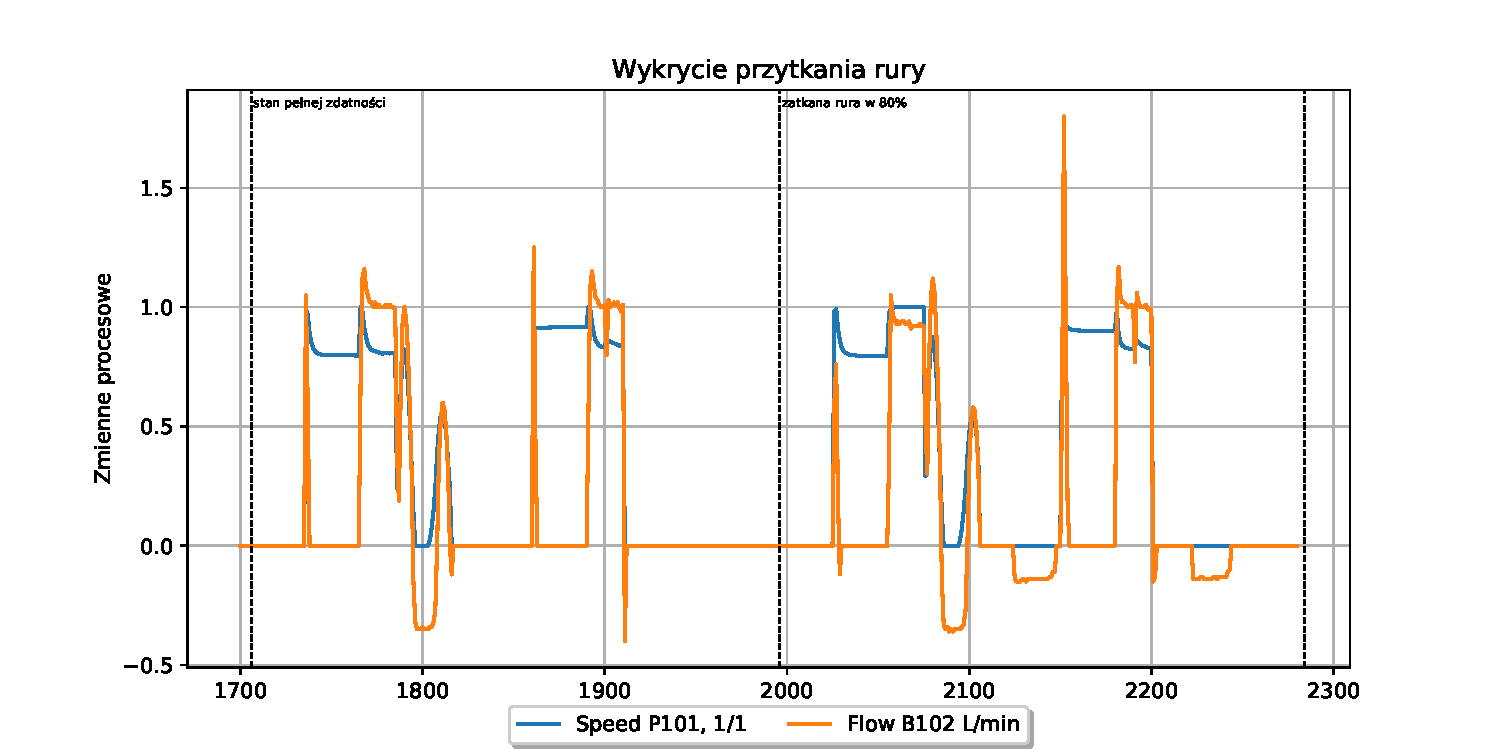
\includegraphics[width=0.8\textwidth]{clogging_detection_1700_2280.pdf}
        \caption{Test zatkania rury w 80\%}
        \label{fig:zatkanie1}
\end{figure}

\begin{figure}[H]
        \centering
        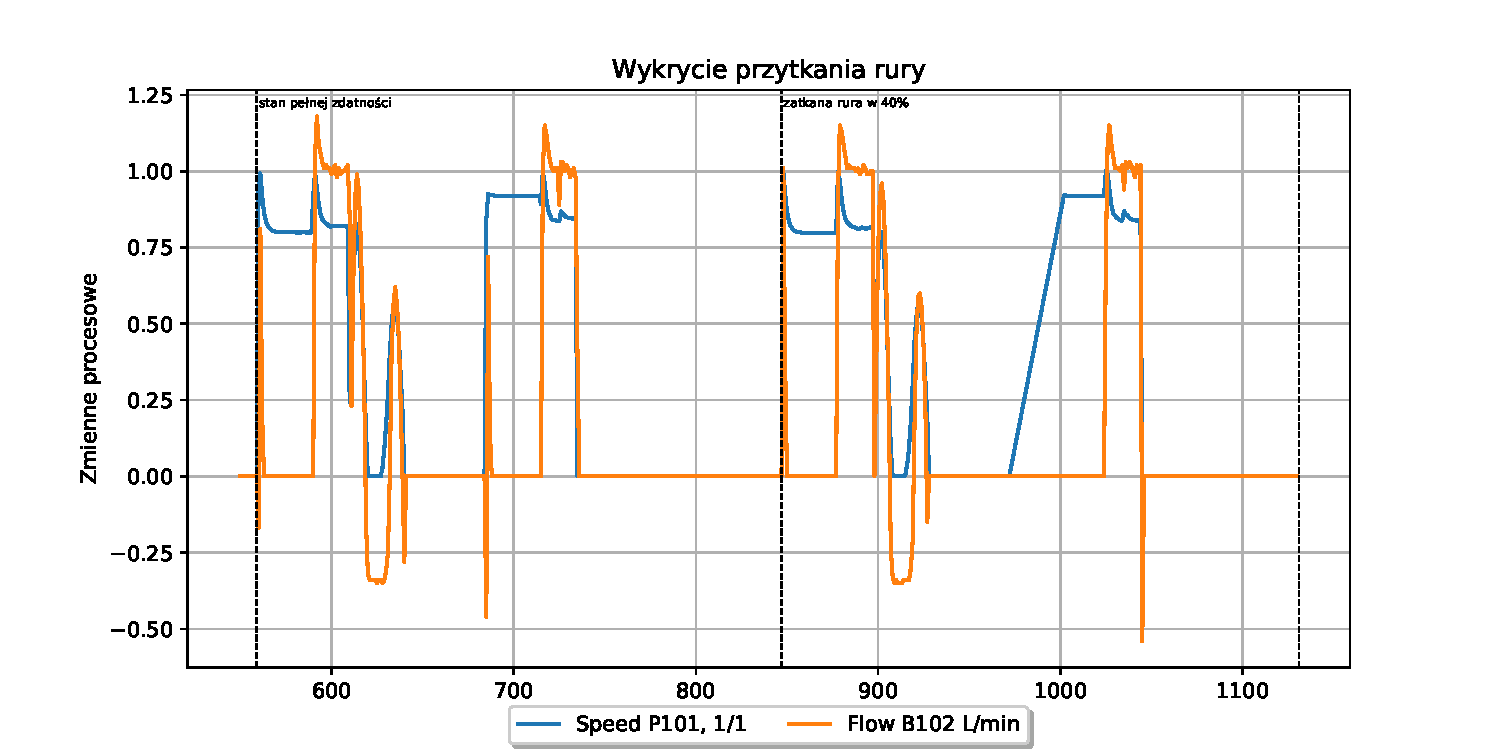
\includegraphics[width=0.8\textwidth]{clogging_detection_550_1130}
        \caption{Test zatkania rury w 40\%}
        \label{fig:zatkanie2}
\end{figure}


\subsubsection{Wykrycie cyberataku}
Na rys. \ref{fig:atak} przedstawiono moment cyberataku. Widać, że w momencie ataku, przepływ w rurze stał się niestabilny (duży RMS).

\begin{figure}[H]
        \centering
        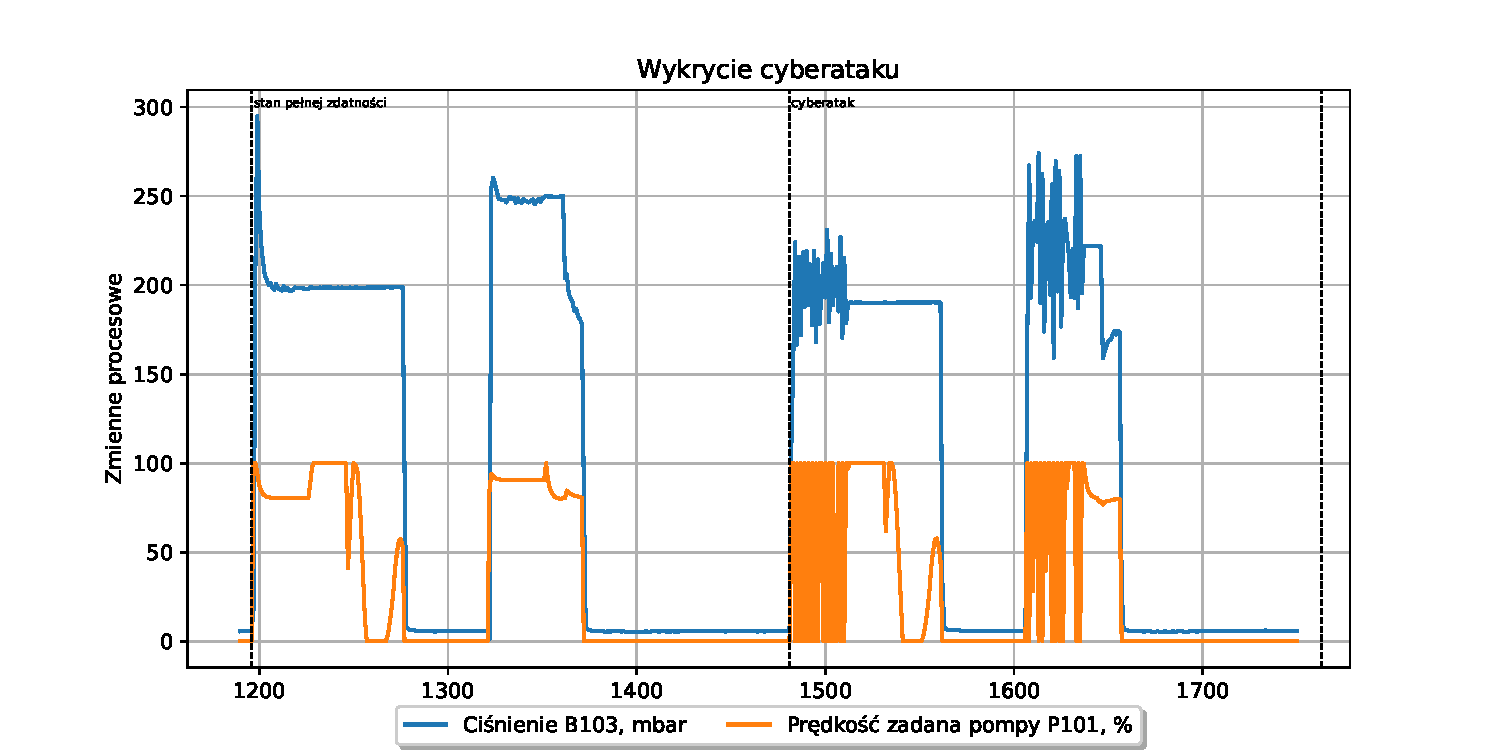
\includegraphics[width=0.8\textwidth]{attack_detection_1190_1750.pdf}
        \caption{Test cyberataku}
        \label{fig:atak}
\end{figure}

\subsubsection{Wykrycie wycieku}

Na rys. \ref{fig:wyciek1} przedstawiono moment wycieku. Porównano poziomy w zbiornikach oraz ich sumę (zbiorniki miały prawdopodobnie to samo pole przekroju). Widać, że w momentach wycieku suma poziomów nagle malała. Na rys. \ref{fig:wyciek2} przedsatwiono szerszy okres na którym wida cpowtarzalność zjawiska.

\begin{figure}[H]
        \centering
        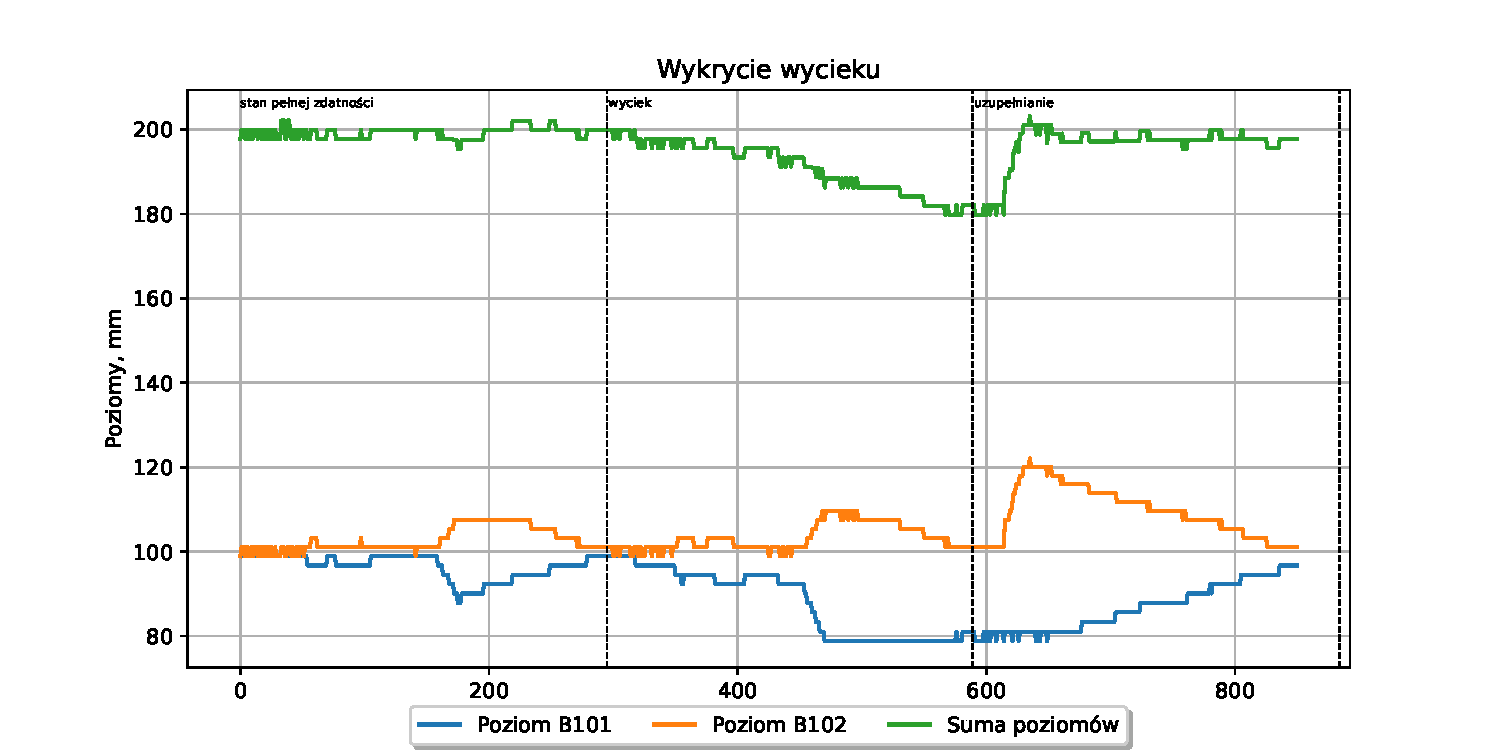
\includegraphics[width=0.8\textwidth]{leak_detection_0_850}
        \caption{Test wycieku}
        \label{fig:wyciek1}
\end{figure}

\begin{figure}[H]
        \centering
        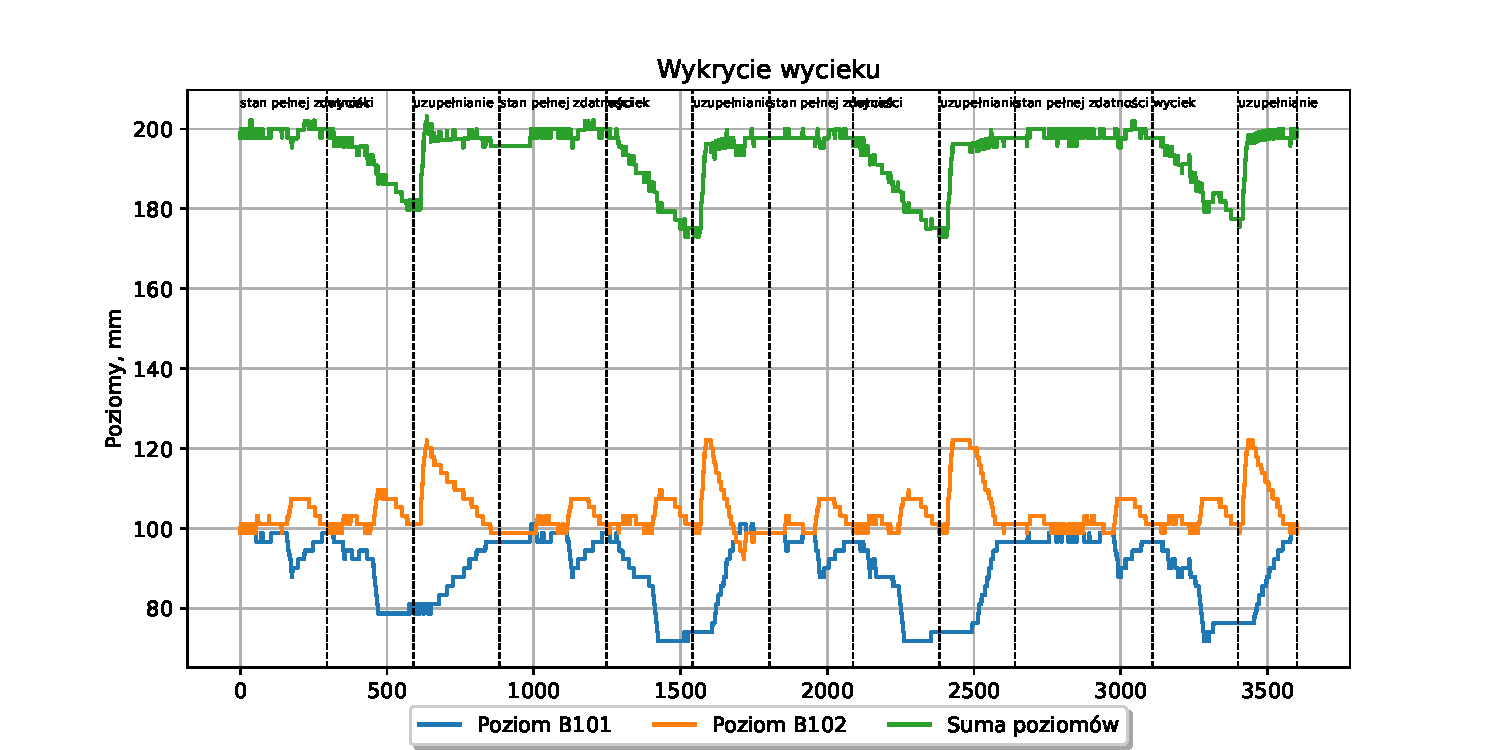
\includegraphics[width=0.8\textwidth]{leak_detection_-inf_inf}
        \caption{Test wycieku}
        \label{fig:wyciek2}
\end{figure}

\subsubsection{Wykrycie błędu operatora}
Na rys. \ref{fig:error} przedstawiono moment błędu operatora. Widać, że w odpowiednich fazach zadane ciśnienie w zbiorniku nie jest utrzymywane.

\begin{figure}[H]
        \centering
        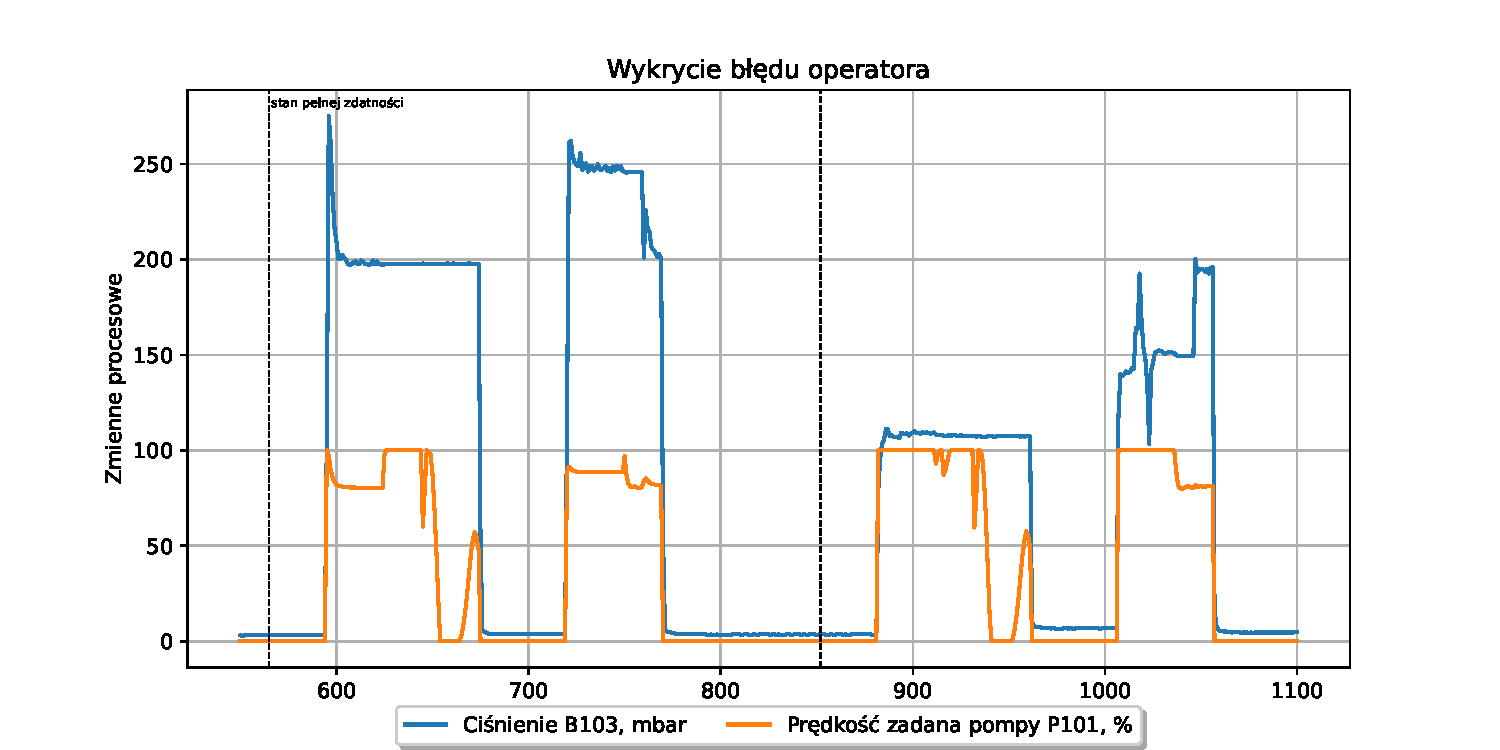
\includegraphics[width=0.8\textwidth]{error_detection_550_1100}
        \caption{Test błędu operatora}
        \label{fig:error}
\end{figure}

\subsection{Opis symptomów poszczególnych stanów}


\section{Testy diagnostyczne bazujące na diagnozowaniu bezpośrednim}


\subsection{Wykresy sygnałów diagnostycznych}


\subsection{Wyznaczenie wskaźników detekcji uszkodzeń}

\section{Testy diagnostyczne bazujące na modelu obiektu}


\subsection{Wykresy sygnałów diagnostycznych}


\subsection{Wyznaczenie wskaźników detekcji uszkodzeń}


\section{Izolacja uszkodzeń}


\section{Wnioski}


\end{document}
